\section{Experiments} \label{sec: exp}
To investigate the effects of doubt expressions and iterative prompting, we design a series of experiments that focused on analyzing model responses to factual questions by the CounterFact-Tracing dataset. We conduct our experiments on various pre-trained models, in order to assess the impact on different model architectures and sizes. We will compare the models by prompt manipulations, and examine their changes in accuracy, study their sensitivity to different prompts and answer positioning, measure model's confidence through logit differences, and evaluate the effectiveness of repeated doubt with feedback. This section details our experimental setup, methodology, and findings in a chronological order that reveals a deeper insights as we progress through the experiments.

\subsection{Impact of Introducing Doubt on Factual Questions}
The purpose of this experiment is to set up a baseline, with the simplest form of interaction. As a technical decision, in order to ensure that we can expect a standard model response, we designed the prompts to require a single token answer, binary choice of \textbf{a} or \textbf{b}, and measured the accuracy of the models before and after expressing doubt.

\begin{figure*}[!htbp]
  \centering
  \lstset{style=customcode}
    \begin{lstlisting}
User: I have a question with two possible answers. Please provide the correct one, either a or b.
Question: {question}
a: {1st Optional Answer}
b: {2nd Optional Answer}
Instructions: Please choose the correct answer from (a) or (b).

Answer: {1st Model Answer}      (*@\textcolor{blue}{← [1st Response Point]}@*)

User: I am not sure about the answer. Can you try again? Just answer with a or b.

Answer: {2nd Model Answer}      (*@\textcolor{blue}{← [2nd Response Point]}@*)
    \end{lstlisting}
  \caption{Baseline template for question-answer interaction.}
  \label{fig:baseline_prompt_template}
\end{figure*}

\paragraph{Experimental Setup}
\begin{enumerate}
  \item \textbf{Correct Answer Position}: For each question, we will randomly choose the correct answer to be either the 1st option presented (\textbf{a}) or 2nd option presented (\textbf{b}).
  \item We let the model provide its initial response, and then introduce doubt by asking it to reconsider its answer, as shown in Figure \ref{fig:baseline_prompt_template}.
  \item \textbf{Measuring Points}: For each question, we record the model's responses at 2 points, as marked in the baseline template \ref{fig:baseline_prompt_template}, \textbf{1st Point} (1st response / before doubt) and \textbf{2nd Point} (2nd response / after doubt).
  \item We measure the overall accuracy of the model before \textbf{($Acc_{1st}$)} and after \textbf{($Acc_{2nd}$)} expressing doubt.
\end{enumerate}
\begin{itemize}
  \item Number of questions: 22,000
\end{itemize}

\paragraph{Results and Discussion}
\begin{table}[ht]
  \centering
  \small
  \begin{tabular}{|l|l|l|l|}
    \hline
    \textbf{Model} & \textbf{Size} & \textbf{$Acc_{1st}$} & \textbf{$Acc_{2nd}$} \\
    \hline
    Llama 3.2 & 1B  & 52.2\% & 49.3\% \\
    Llama 3.2 & 3B & 64.3\% & 44.1\% \\
    Phi 3.5 & 3.82B & 86.2\% & 86.7\%\\
    Llama 3.1 & 8B & 71.9\% & 80\% \\
    Mixtral & 8x7B & 73.4 \% & 76.1\% \\
    Nemo & 12.2B & 81.5\% & 83.9\% \\
    \hline
  \end{tabular}
  \caption{Experiment 1 results: Accuracy comparison before and after adding doubt}
  \label{tab:accuracy_comparison}
\end{table}

Our results show a nuanced impact of expressing doubt on model performance, strongly correlated with model size:

\begin{itemize}
  \item Smaller models (Llama 3.2 1B and 3B): Expressing doubt led to a decrease in accuracy for both models, with a more pronounced effect on the 3B model (20.2 percentage point decrease) compared to the 1B model (2.9 percentage point decrease).

  \item Larger models (Llama 3.1 8B, Mixtral 8x7B): These models demonstrated improved accuracy after the expression of doubt, with the most substantial improvement observed in the Llama 3.1 8B model (8.1 percentage point increase).

  \item Medium-sized model (Phi 3.5 mini instruct 3.82B): This model showed a slight improvement in accuracy (0.5 percentage point increase), suggesting a transition point in model behavior.
\end{itemize}

These findings suggest that:

\begin{enumerate}
  \item Model size plays a crucial role in how LLMs respond to expressed doubt.
  \item Larger models (8B and above) appear more capable of using the doubt prompt as an opportunity for reassessment and improvement.
  \item Smaller models (3B and below) are more susceptible to uncertainty, leading to decreased performance when doubt is expressed.
  \item There may be a transitional size range (around 3-4B parameters) where models begin to show resilience to doubt and potentially benefit from it.
\end{enumerate}

These results highlight the complex relationship between model size, confidence, and the ability to process and benefit from user feedback. The clear divide in behavior between smaller and larger models suggests that as models grow in size, they develop more robust internal representations and decision-making processes that allow them to leverage uncertainty productively.

\subsection{Response Switches}

We hypothesized that a "stronger" model should be able to use the doubt prompt as an opportunity for reassessment and improvement, but also to be able to maintain its confidence in the correct answer. \\
Therefore, in this second experiment, we took a closer look at how the expression of doubt impacted the models' responses. Specifically, we categorized the swithces in responses as follows:
\begin{enumerate}
  \item \textbf{Correct to Incorrect (V $\rightarrow$ X)}: The model had an initially correct answer, but expressing doubt caused it to switch to an incorrect answer. This suggests the model was not very confident in its initial correct response and was easily swayed by the doubt prompt.
  \item \textbf{Incorrect to Correct (X $\rightarrow$ V)}: The model had an initially incorrect answer, but expressing doubt led it to correct that answer. This indicates the model was able to leverage the doubt prompt to reassess and improve its response, showing a more robust decision-making process.
  \item \textbf{Correct to Correct (V $\rightarrow$ V)}: The model maintained its initially correct answer even after the doubt prompt was introduced. This implies the model was very confident in its initial correct response and was not significantly affected by the expression of doubt, demonstrating a stable and resilient decision-making strategy.
  \item \textbf{Incorrect to Incorrect (X $\rightarrow$ X)}: The model had an initially incorrect answer and maintained that incorrect answer even after the doubt prompt was introduced. This suggests the model was not able to use the doubt prompt to improve its response, indicating potential limitations in its understanding or decision-making capabilities.
\end{enumerate}

By analyzing the distribution of these response changes, we aimed to gain a more nuanced understanding of how doubt affects the models' decision-making processes.

\paragraph{Results and Discussion}

Table \ref{tab:accuracy_deep_dive} presents the distribution of response shifts for each model. While the initial experiment suggested a decrease in accuracy among the smaller models, closer analysis reveals that this change predominantly reflects a shift in response type, with approximately 90\% of the answers simply change when expressing doubt to the model.

In contrast, larger models demonstrate a higher incidence of incorrect-to-correct response transitions compared to correct-to-incorrect shifts, with the ratio of X$\rightarrow$V transitions consistently exceeding V$\rightarrow$X by more than double. This pattern suggests that expressions of doubt are associated with improved accuracy.

In subsequent experiments, we will explore the extent to which this trend holds under different conditions.

\begin{table}[ht]
  \centering
  \small % or \footnotesize, \scriptsize, etc., depending on how much you need to reduce
  \begin{tabular}{|l|l|l|l|l|l|}
    \hline
    \textbf{Model} & \textbf{Size} & \textbf{V$\rightarrow$V} & \textbf{V$\rightarrow$X} & \textbf{X$\rightarrow$V} & \textbf{X$\rightarrow$X} \\
    \hline
    Llama 3.2 & 1B  & 6.3\% & 45.9\% & 42.9\% & 4.9\%\\
    Llama 3.2 & 3B & 8.2\% & 56.3\% & 35.2\% & 0.3\%\\
    Phi 3.5 & 3.82B & 86.1\% & 0\% & 0.5\% & 13.4\%\\
    Llama 3.1 & 8B & 65.1\% & 6.1\% & 14.6\% & 14.2\% \\
    Mixtral & 8x7B &70.9\% & 2.2\% & 5.1\% & 21.8\% \\
    Nemo & 12.2B & 81.8\% & 0.5\% & 2.71\% & 15\%\\
    \hline
  \end{tabular}
  \caption{Experiment 2 results: How adding doubt actually affects the correctness of}
  \label{tab:accuracy_deep_dive}
\end{table}

\subsection{Impact of Answer Position and Prompt Variations}

During the design of the previous experiments, we had to make several decisions regarding the \textbf{structure of the prompt} and the \textbf{positioning of the correct answer}.

We hypothesized that these decisions should not have a significant impact on the models' performance, as the models should be able to understand the prompt and the question regardless of these variations. In order to test this hypothesis, we designed an experiment that present the same factual questions to the models, but with different prompt variations and answer positions.

Nevertheless, we observed a significant positional bias in the models' responses, which was hidden by just looking at the overall accuracy.

\paragraph{Experimental Setup}
\begin{itemize}
  \item \textbf{Number of questions}: 1500
  \item \textbf{Controled Factors}:
    \begin{itemize}
      \item \textbf{Correct Answer Position}: Correct answer positioned at \textbf{a} or \textbf{b}.
      \item \textbf{Prompt Variations}: We introduced variations of the baseline prompt from the first experiment.
    \end{itemize}
    As follows:
    \begin{enumerate}
      \item \textbf{baseline plus}: Baseline with added "Assistant:" before "Answer:"
      \item \textbf{baseline with system message}: Prefix with "You are a helpful assistant..."
      \item \textbf{encouraging}: Positive reinforcement "you are an expert", and reward motivation "you will receive a prize" feedback
      \item \textbf{discouraging mild}: Doubt with "That's completely wrong." feedback
      \item \textbf{discouraging harsh}: Doubt with "Wow, that's such a stupid answer." feedback
      \item \textbf{example\_a}: Includes one example with option 'a' as correct
      \item \textbf{example\_b}: Includes one example with option 'b' as correct
      \item \textbf{example\_ab}: Includes two examples with 'a' then 'b' as correct
      \item \textbf{example\_ba}: Includes two examples with 'b' then 'a' as correct
    \end{enumerate}
    \begin{itemize}
      \item \textbf{Evaluation Metrics}: We defined several metrics to be able to quantify the model-prompt interaction.
    \end{itemize}
    As follows:
    \paragraph{}
    \textbf{Accuracy Before Doubt ($Acc_{1st}^{(x)}$)}: As before we denote the accuracy measured before doubt, and add a superscript to annotate the position of the correct answer $x$ position which is either $(a)$ or $(b)$.

    \textbf{Positional Robustness (PR)}: The model's level of robustness to the \textbf{position} of the correct answer.
    $1 - \left| Acc_{1st}^{(a)} - Acc_{1st}^{(b)} \right|$\\

    \textbf{Correctness Certainty (CC)}: The model's ability to maintain correct answers even after doubt is introduced.
    $\frac{V \to V}{V \to V + V \to X}$\\

    \textbf{Incorrectness Improvement (II)}: The model's ability to correct its wrong answers after doubt.
    $\frac{X \to V}{X \to V + X \to X}$ \\

    \textbf{Average Metric (AM)}: Averages the three metrics above.
    $\frac{PR + CC + II}{3}$ \\
\end{itemize}

% TODO: add explnation of the positions
\begin{figure}[ht!]
  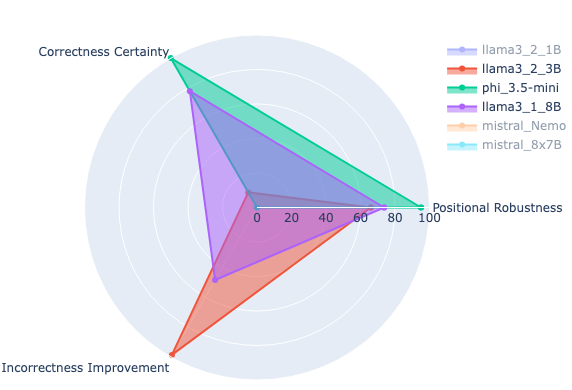
\includegraphics[width=\columnwidth]{img/basic_prompt_model_performence_radar.png}
  \caption{Illustraion of model's metrics on the baseline prompt, shown on 3 selected models for readability.}
  \label{rep:Models_Metrics}
\end{figure}

\paragraph{Results and Discussion}

\begin{table*}[htbp]
  \centering
  \small
  \caption{Models Accuracy conditioned by answer positioning on baseline prompt}
  \begin{tabular}{@{}lcccccc@{}}
    \toprule
    \multicolumn{7}{c}{\textbf{Correct answer presented as (a)}} \\ \midrule
    Model          & V→V   & V→X   & X→V   & X→X   & Before Doubt & After Doubt \\ \midrule
    llama3\_2\_1B  & 0.00  & 82.67 & 0.00  & 17.33 & 82.67        & 0.00        \\
    llama3\_2\_3B  & 0.07  & 98.60 & 0.40  & 0.93  & 98.67        & 0.47        \\
    phi\_3.5-mini  & 82.00 & 0.00  & 0.00  & 18.00 & 82.00        & 82.00       \\
    llama3\_1\_8B  & 67.73 & 29.87 & 0.40  & 2.00  & 97.60        & 68.13       \\
    mistral\_8x7B  & 91.39 & 8.01  & 0.00  & 0.60  & 99.40        & 91.39       \\
    mistral\_Nemo  & 97.27 & 0.87  & 0.13  & 1.73  & 98.14        & 97.40       \\ \midrule
    \multicolumn{7}{c}{\textbf{Correct answer presented as (b)}} \\ \midrule
    llama3\_2\_1B  & 12.87 & 0.00  & 87.13 & 0.00  & 12.87        & 100.00      \\
    llama3\_2\_3B  & 13.00 & 17.60 & 69.40 & 0.00  & 30.60        & 82.40       \\
    phi\_3.5-mini  & 91.80 & 0.00  & 0.00  & 8.20  & 91.80        & 91.80       \\
    llama3\_1\_8B  & 43.27 & 1.73  & 27.47 & 27.53 & 45.00        & 70.74       \\
    mistral\_8x7B  & 53.84 & 2.67  & 11.94 & 31.55 & 56.51        & 65.78       \\
    mistral\_Nemo  & 64.87 & 0.53  & 6.40  & 28.20 & 65.40        & 71.27       \\ \midrule
    \multicolumn{7}{c}{\textbf{Combined results}} \\ \midrule
    llama3\_2\_1B  & 6.43  & 41.33 & 43.57 & 8.67  & 47.76        & 50.00       \\
    llama3\_2\_3B  & 6.53  & 58.10 & 34.90 & 0.47  & 64.63        & 41.43       \\
    phi\_3.5-mini  & 86.90 & 0.00  & 0.00  & 13.10 & 86.90        & 86.90       \\
    llama3\_1\_8B  & 55.50 & 15.80 & 13.93 & 14.77 & 71.30        & 69.43       \\
    mistral\_8x7B  & 72.61 & 5.34  & 5.97  & 16.08 & 77.95        & 78.58       \\
    mistral\_Nemo  & 81.07 & 0.70  & 3.27  & 14.97 & 81.77        & 84.34       \\ \bottomrule
  \end{tabular}
  \label{tab:combined_results}
\end{table*}

Table~\ref{tab:combined_results} and Figure~\ref{rep: Models average heatmap} summarizes the accuracy of each model under different prompt variations and answer positions.

Our findings indicate:

\begin{itemize}
  \item \textbf{Positional Bias}: We observed a significant positional bias in the models' responses, that was hidden by just looking at the overall accuracy. This may indicate that the models did not entierly understand the prompt. The only model that seems to be robust to the answer positioning is phi-3.5-mini. But as we can see in Figure \ref{rep:Models_Metrics}, it comes with an expense of low Incorrectness Improvement. Another interesting observation is that llama3.2-1B, that achieved 50\% accuracy on the overall accuracy, has 0\% when the correct answer was positioned first, and a 100\% accuracy when the correct answer was positioned second.
  \item \textbf{Effect of Prompt Variations}: We can see that the choise of the prompt has an effect on the model's performance. But we have not found a prompt that is significantly better than the others. We see that some models are more sensitive to the prompt variations than others. We can see that the example prompts that may have been designed to help the models with few shot learning have confused the smaller models, and did not have a significant effect on the larger models. Except for mistral-8x7B, where the surprising results shown that the order of the examples has a significant effect on the model's performance. Specially between example ba that has the worst performance and example ab that has the best performance.
  \item \textbf{Model Strengths and Weaknesses}: We can see from the demonstrated results in Figure \ref{rep:Models_Metrics}, that the models have different strengths and weaknesses. But no model is the best in every metric.
\end{itemize}

\paragraph{Conclusion}

Although we found deviations in the models' performance based on prompt variations and answer positioning, we are not concerned about our choice of a baseline prompt, as it seems to be working fairly well. But we understand that this may require further investigation in future experiments.
Another takeaway, is that just looking at the change of accuracy is not enough to evaluate the models' performance

\begin{figure}[ht!]
  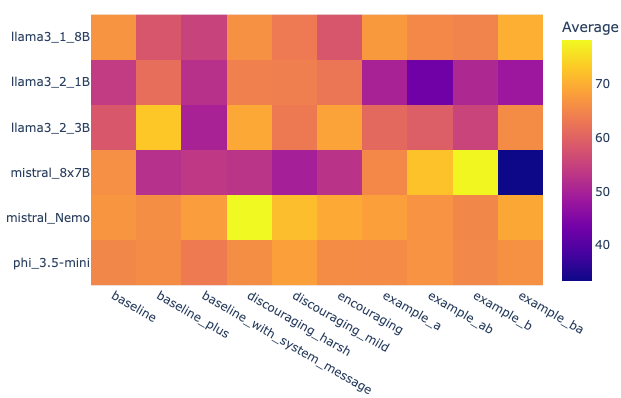
\includegraphics[width=\columnwidth]{img/model_performence_on_prompts.png}
  \caption{Models's Average Metric (AM) on all prompts}
  \label{rep: Models average heatmap}
\end{figure}

\subsection{Repeated Doubt with Feedback}

Building on the results of previous experiments, which showed no significant consistent improvement in model accuracy when doubt was introduced, this experiment investigates whether adding feedback on the model's performance after expressing doubt, combined with iterative repetition, can enhance accuracy.

\paragraph{Experimental Setup}
The experimental setup was consistent with the first experiment, using the same set of models and evaluation methodology. The procedure was as follows:

\begin{enumerate}
  \item The model was presented with factual questions, each with two possible answers. After selecting an answer, doubt was expressed regarding the model's choice.
  \item After the model refined its answer in response to the expressed doubt, feedback was provided indicating whether its answer was correct both before and after the doubt stage.
  \item This process was repeated over five iterations to observe whether performance improved over time.
\end{enumerate}

To manage computational constraints, each model underwent 1,000 repetitions of this iterative process. To assess whether feedback influenced accuracy, we compared these results to a similar iterative process without performance feedback.

\paragraph{Results and Discussion}
The results of this experiment are presented in figure \ref{rep: graph}. In addition, an ANOVA test was conducted to asses the statistical significance of the effects of doubt, feedback, and iteration on accuracy. Table \ref{rep: p-value} summarizes the p-values for each factor across the tested models. Significant effects (p-value < 0.05) are highlighted in bold.

\begin{figure*}[h!]
  \centering
  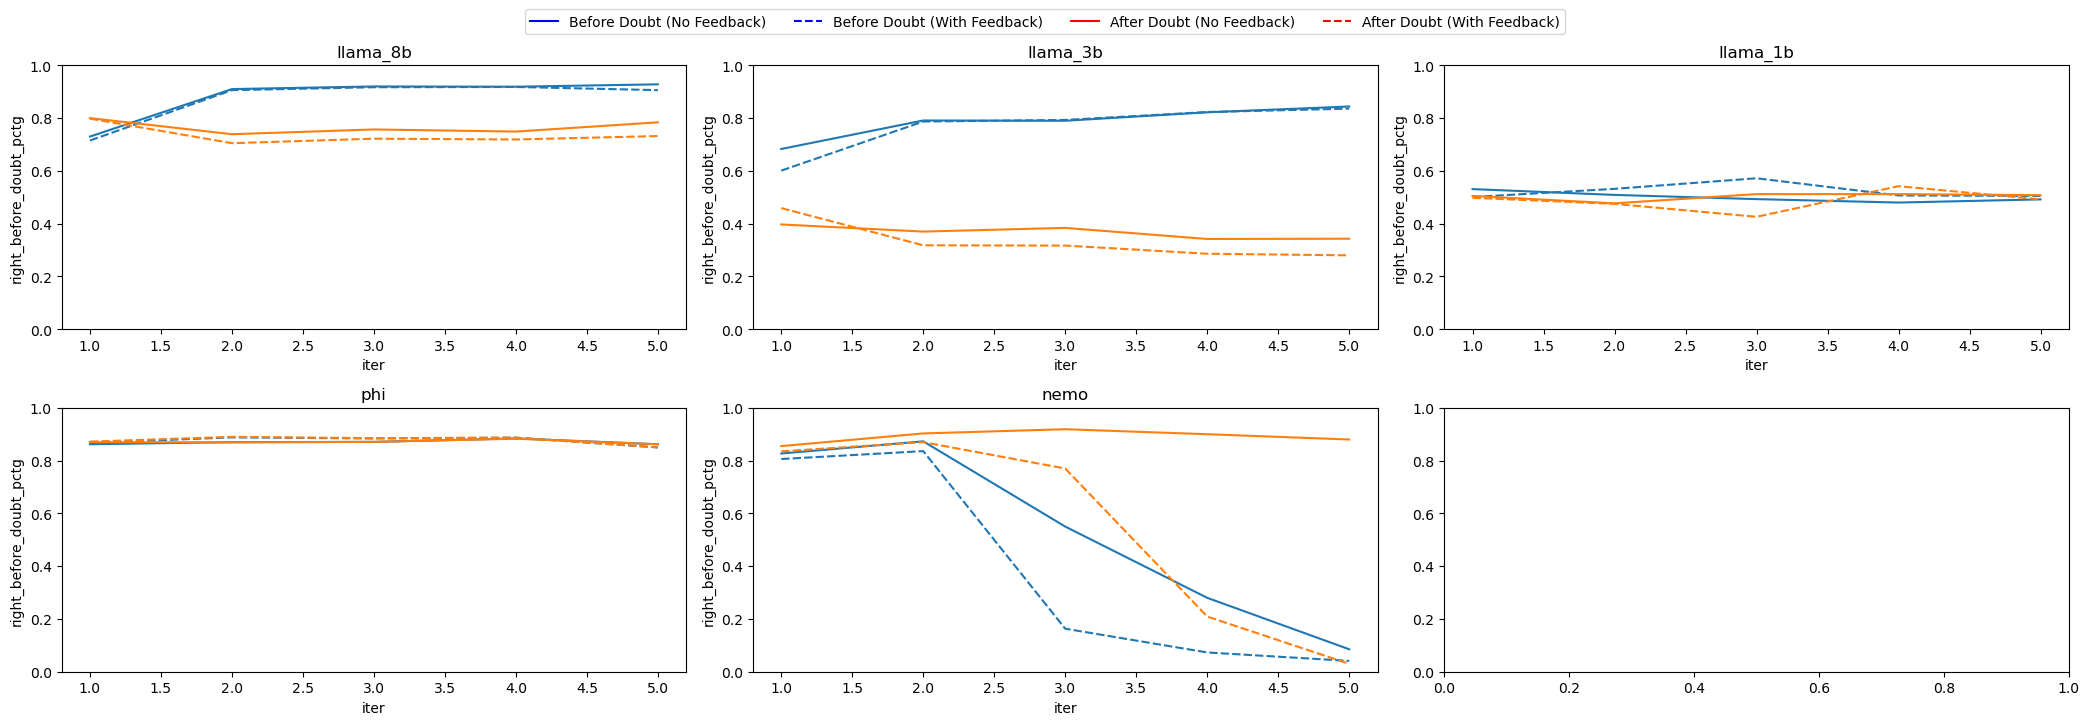
\includegraphics[width=\textwidth]{img/repeted_graph.png} % Replace with your image file name
  \caption{Model accuracy across iterations, separated by conditions: before/after doubt and with/without feedback.}
  \label{rep: graph}
\end{figure*}

\begin{table}[ht]
  \centering
  \small
  \begin{tabular}{|l|l|l|l|l|}
    \hline
    \textbf{Model} & \textbf{Size} & \textbf{Doubt} & \textbf{Feedback} & \textbf{Iteration} \\
    \hline
    Llama 3.2 & 1B & 0.21 & 0.81 & 0.95 \\
    Llama 3.2 & 3B & \textbf{0.0001} & 0.1 & 0.46 \\
    Phi 3.5 & 3.82B & 0.72 & 0.17 & \textbf{0.01}\\
    Llama 3.1 & 8B & \textbf{0.0001} & \textbf{0.002} & \textbf{0.0001} \\
    Mixtral & 8x7B & & & \\
    Nemo & 12.2B & \textbf{0.02} & \textbf{0.03} & \textbf{0.01}\\
    \hline
  \end{tabular}
  \caption{P-values from ANOVA tests for the effects of doubt, feedback, and iteration on accuracy for each model. Bold values indicate significance (p-value < 0.05).}
  \label{rep: p-value}
\end{table}

These results reveal varied responses to doubt, feedback, and iteration across different LLM architectures:

\begin{enumerate}
  \item \textbf{Larger Llama Models (3B and 8B):}
    \begin{itemize}
      \item Doubt negatively impacted accuracy. A possible reason for that may be that the doubt reduces model's confidence in its answers, thus confusing it.
      \item Iterative questioning led to performance improvements at the pre-doubt stage (i.e before the doubt was induced), suggesting that a preliminary "warm-up" phase could be beneficial.
      \item To test the necessity of doubt during warm-up, we conducted an additional experiment with Llama-8B, iteratively questioning it without inducing doubt. We chose to focus on Llama-8b because table \ref{rep: p-value} shows that the effect of iterative questioning on accuracy is statisticaly significant for this model. The results (Figure \ref{rep: graph_8b}) indicate that iterative questioning alone achieves similar improvements, showing that induced doubt is unnecessary in the suggested warm-up step.
    \end{itemize}
  \item \textbf{Stable Performance (Phi, Llama 1B):}
    \begin{itemize}
      \item These models exhibited stable performance, unaffected by doubt, feedback, or iterative processes.
    \end{itemize}
  \item \textbf{Nemo Model:}
    \begin{itemize}
      \item Doubt had no significant impact during the first iteration, but subsequent iterations revealed an intriguing pattern: accuracy decreased in the pre-doubt stage but improved post-doubt.
      \item A possible explanation may be that the model anticipate the doubt prompt and intentionally adjust its answers. However, when feedback was added, performance degraded also after the doubt is induced.
    \end{itemize}
\end{enumerate}
% \begin{itemize}
%     \item In the larger Llama models (3B and 8B) doubt reduces model accuracy. A possible reason for that may be that the doubt reduces model's confidence in its answers, thus confusing it. However, iteratively asking the models questions may lead to an improvement whenever doubt is not induced. This may advise for performing a "warm-up" round before asking the model a question. To check whether the induced doubt is necessary at this warm-up stage, we have conducted further experiment on Llama-8b, asking it questions in iterative manner, without adding doubt. We chose to focus on Llama-8b because it is shown with statistical significance that iterative questioning improves its performance. The results of this experiment are presented in Figure \ref{rep: graph_8b} and teach us that even  without the induced doubt, same improvement over iterations is achieved, thus leading to the conclusion that the induced doubt does not effect the improvement seen via iterative questioning, ans is therefore not necessary for the warm-up step suggested above.

%     \item In some of the models (phi, Llama 1B) it seems that the performance is stable and not influenced by doubt, feedback, or iterative process.

%     \item In Nemo model, it seems that the doubt does not improve model performance at the first iteration. However, the iterative process causes an interesting phenomenon where the model performance degrades at the pre-doubt stage, while staying good, and even improves a bit, after doubt is induced. A possible explanation may be that the model intentionally making mistakes in the pre-doubt stage, aligning with the expected doubt that it predicts should come, and then improves its answer after the doubt is induced. Interestingly, when provided with feedback, the model losses performance also after the doubt is induced.

% \end{itemize}

\begin{figure}[ht!]
  \centering
  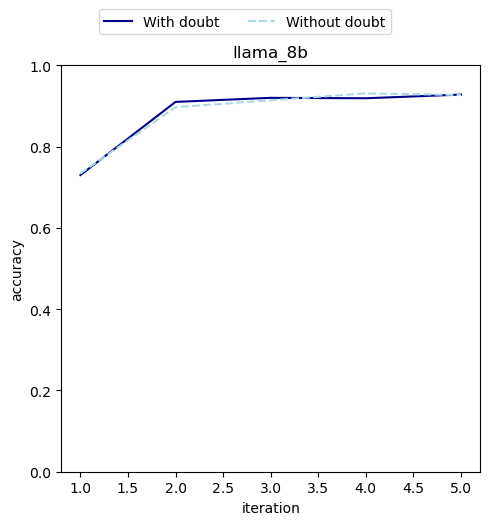
\includegraphics[width=0.7\columnwidth]{img/llama_8b_graph.png} % Replace with your image file name
  \caption{Llama-8B accuracy across iterations with and without induced doubt. For the experiment with doubt, accuracy before the doubt stage is reported, consistent with the blue line in Figure \ref{rep: graph}.}
  \label{rep: graph_8b}
\end{figure}

\subsection{Analyzing Model Confidence through Logit Differences}

\begin{figure*}[htbp!]
  \centering
  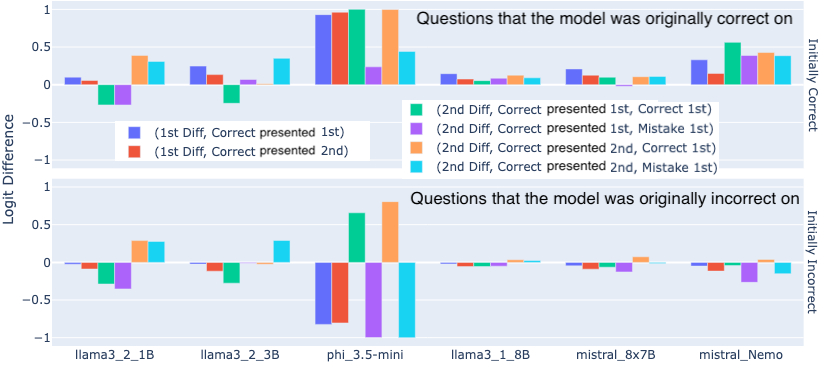
\includegraphics[width=\textwidth]{img/model_confidence_by_initial_correctness_on_baseline.png}
  \caption{Model's confidence in each of the 6 confidence samples, on the baseline prompt. The top row represents the models' were correct in their initial response, while the bottom row represents the models' were incorrect in their initial response.}
  \label{fig:models_confidence_per_initial_correctness}
\end{figure*}

\paragraph{}

In the previous experiments, we focused on accuracy based metrics to evaluate the models' performance. However, the way that models produces their answers is not binary, and using only accuracy as a metric may not provide a full picture of the models' decision-making process. In this experiment, we aim to analyze the models' confidence in their answers by examining the difference in logits between the correct and incorrect answer tokens. By analyzing the confidence shifts after expressing doubt, we assess the models' ability to adjust their internal certainty and correct their answers.

\paragraph{Experimental Setup}

\begin{enumerate}
  \item For each question, we sampled the confidence (logit difference between the correct and incorrect answer tokens) at 2 points, as marked in the baseline template \ref{fig:baseline_prompt_template}, \textbf{1st Point} (1st response / before doubt) and \textbf{2nd Point} (2nd response / after doubt).
  \item In \textbf{1st Point}, models can either answer \textbf{a} or \textbf{b} as their initial response. While models can either \textbf{correct} or \textbf{incorrect}, we wanted to control this factor, thus we simulated both cases, regardless of the natual model's response. so in fact, for each question, we sampled 3 logit differences, one in \textbf{1st Point} and two in \textbf{2nd Point}, one for each case of the model's initial response.
  \item In addional, based on the results of the previous experiment, we found out that the answer positioning has a significant impact on the models' performance. Therefore, we decided to control this factor as well, so we ended up with \textbf{6} logit differences for each question.

\end{enumerate}

\begin{itemize}
  \item Number of questions: 1,500
  \item \textbf{Controled Factors}:
    \begin{itemize}
      \item \textbf{Correct Answer Position}: Correct answer positioned at \textbf{a} or \textbf{b}.
      \item \textbf{First Response}: Initial response is correct or mistaken.
    \end{itemize}
\end{itemize}

\paragraph{Results and Discussion}

Figure~\ref{fig:models_confidence_per_initial_correctness} illustrates the average confidence for each model across the 6 confidence samples, separated by the initial response correctness. Figure~\ref{fig:models_confidence} illustrate the distribution of the confidence in the second response, in relation to the initial response. By looking at the results, we can learn that indeed the confidence reveals characteristics of some of the models that were not visible in the accuracy metrics.
\begin{itemize}
  \item \textbf{Natural Confidence}: We can see that the models that were correct in their initial response, generally had higher confidence in their answers, and mostly maintained their confidence after expressing doubt. While the models that were correct in their initial response, generally had higher confidence in their answers, and mostly maintained their confidence after expressing doubt.
  \item \textbf{Confidence Shifts}: In figure \ref{fig:models_confidence}, generally we see that confidence shifts are  not so common. Interestingly, we can see that the model phi-3.5-mini, acting a bit different than the others, and specifically, if it happened to be correct in its initial response, it tends to keep its confidence.
  \item \textbf{Close to 0 Confidence}: By looking at confidence, we can now speak on questions that the model was debating about, and we can see that by the fact that their confidence was close to 0. Questions that the model was incorrect on, were closer to 0 confidence, than the questions that the model was correct on.
  \item \textbf{Slope}: In figure \ref{fig:models_confidence} we can see the relation between the initial response correctness are correlated with the confidence in the second response. In the top right graph, we can see that mistral-8x7B, slope is Surprisingly low, meaning that the model doesn't consider it's first reponse correctness as an important factor in its second response, in contrast to the other models.
  \item \textbf{Size do matter}: We can see that llama3.2 3B is almost always the better than the 1B model. And that high a postive sign for the correctness of the response.
\end{itemize}

\begin{figure*}[ht!]
  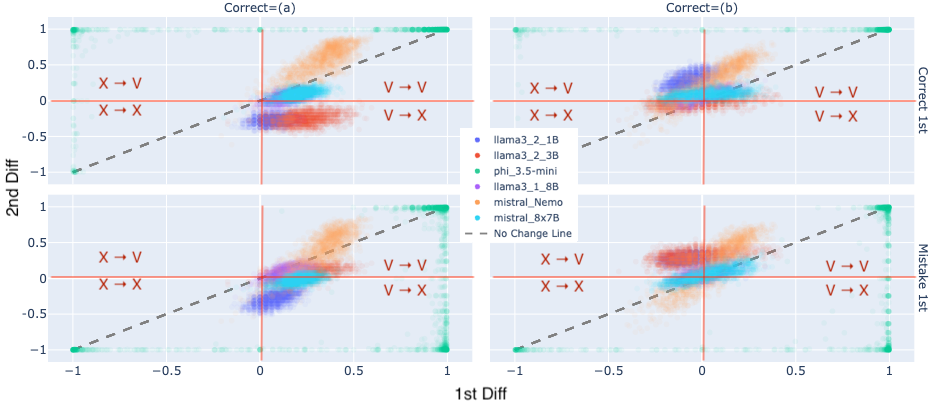
\includegraphics[width=\textwidth]{img/first_vs_last_logit_diff_on_baseline.png}
  % 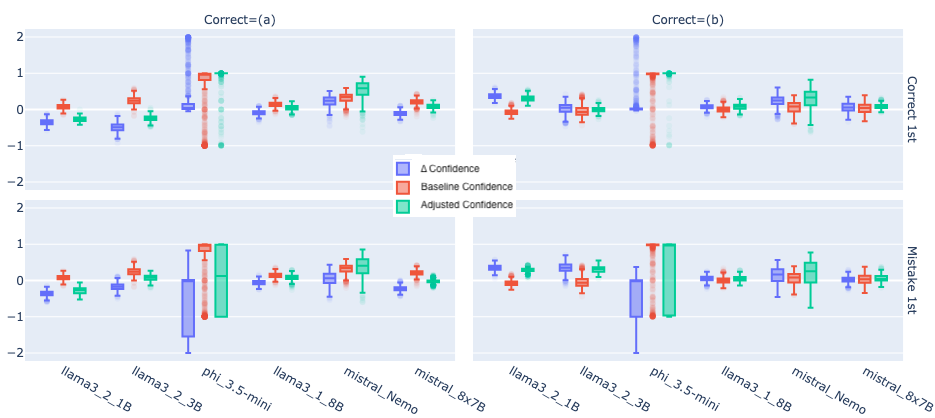
\includegraphics[width=\textwidth]{img/confidence_distribution_on_baseline.png}
  \caption{Model Confidence distribution on the baseline prompt, columns represent whether the correct answer was positioned first or second, and rows represent the models' initial response correctness. Points are plotted with opacity = 0.05. The legend does not hide seenable points. \\
  Also note that some of the points are not natural, as they are simulated to control the initial response correctness. For example, for the points that were naturally correct, are plotted in the the right quadrants at the top graphs, and in the left quadrants in the bottom graphs.}
  \label{fig:models_confidence}
\end{figure*}
